\documentclass[10pt, a4paper, italian]{article}
\usepackage[T1]{fontenc}
\usepackage[utf8]{inputenc}
\usepackage{amsmath, amssymb, amsthm, thmtools, amsfonts, mathtools}
\usepackage{nicefrac}
\usepackage{calc}
\usepackage[pdftex, hyperindex, plainpages=false]{hyperref}
\usepackage[nameinlink]{cleveref} %load before classicthesis (clash)
%\usepackage[nochapters,pdfspacing]{classicthesis}
\usepackage{siunitx}
\usepackage[siunitx]{circuitikz}

\usepackage[a4paper]{geometry}
\usepackage{float}
\usepackage{mdframed}
\usepackage{titling}
\usepackage{booktabs}
\usepackage{graphicx}
\usepackage{caption, subcaption}
\usepackage{xcolor}
\usepackage[italian]{babel}
\usepackage{pgfplots}
\usepackage{listings}
%\usepackage{lmodern}
\usepackage{url}
\usepackage{enumitem}
\usepackage{tikz} %loads after classicthesis (xcolor incompat)

% lets graphicx know path where figures to be included are found
\graphicspath{{../figs/}}
\makeatletter
\def\input@path{{../figs/}}
%or: \def\input@path{{/path/to/folder/}{/path/to/other/folder/}}
\makeatother

% tikz pgf plots setup
\usepgfplotslibrary{external}
\pgfplotsset{compat=1.15}
%\tikzexternalize

% spaces and significant digits/figures for measurements
\sisetup{free-standing-units, space-before-unit, number-unit-product = \;,
scientific-notation = false, round-mode = figures, round-precision = 1,}

% turns all (hyperlinked) references black [default is blue]
\hypersetup{
	linktoc=all,
	colorlinks=true,
	linkcolor=black
}

% code listings config
%\lstset{
%language=Python,
%basicstyle=\ttfamily,
%columns=fullflexible,
%keepspaces=true,
%}

% mdframed (for boxed text) configuration
\mdfsetup{linewidth=0.6pt}

% Default fixed font does not support bold face
\DeclareFixedFont{\ttb}{T1}{txtt}{bx}{n}{12} % for bold
\DeclareFixedFont{\ttm}{T1}{txtt}{m}{n}{12}  % for normal

% Custom colors
\usepackage{color}
\definecolor{deepblue}{rgb}{0,0,0.5}
\definecolor{deepred}{rgb}{0.6,0,0}
\definecolor{deepgreen}{rgb}{0,0.5,0}

% Commands 
\newcommand{\executeiffilenewer}[3]{%
	\ifnum\pdfstrcmp{\pdffilemoddate{#1}}%
		{\pdffilemoddate{#2}}>0%
	{\immediate\write18{#3}}\fi%
}
% input .svg --> .pdf_tex graphs
%\newcommand{\includesvg}[1]{%
%	\executeiffilenewer{#1.svg}{#1.pdf}%
%	{inkscape -z -D --file=#1.svg %
%	--export-pdf=#1.pdf --export-latex}%
%	\input{#1.pdf_tex}%
%}
% Thanks UniPi's Department of Physics E. Fermi
\newcommand{\thanksdf}{(\thanks{Dipartimento di Fisica E.~Fermi,%
Universit\`a di Pisa - Pisa, Italy.}\;)}

% hyperlink to email address
\newcommand{\mail}[1]{\href{mailto:#1}{\textsf{#1}}}

% \vec for bold vectors, instead of overarrows (now "\arrvec")
\let\arrvec=\vec
\renewcommand{\vec}[1]{\boldsymbol #1}
% replaces straight phi with slanted phi
\renewcommand{\phi}{\varphi}
% replaces straight eps with curved epsilon
\newcommand{\eps}{\varepsilon}
% abbreviation for (sub_/super^)scripts of \lim, \sum,... in inline math
\newcommand{\ds}{\displaystyle}

% blackboard/number set letters
\newcommand{\CC}{\mathbb C}
\newcommand{\HH}{\mathbb H}
\newcommand{\KK}{\mathbb K}
\newcommand{\NN}{\mathbb N}
\newcommand{\PP}{\mathbb P}
\newcommand{\QQ}{\mathbb Q}
\newcommand{\RR}{\mathbb R}
\newcommand{\ZZ}{\mathbb Z}

\newcommand{\Abs}[1]{{\left\Vert #1\right\Vert}}
\newcommand{\enclose}[1]{{\left( #1 \right)}}
\newcommand{\Enclose}[1]{{\left[ #1 \right]}}
\newcommand{\floor}[1]{\left\lfloor #1 \right\rfloor}
\newcommand{\ceil}[1]{\left\lceil #1 \right\rceil}
\newcommand{\To}{\rightrightarrows}

% Math operators
\DeclareMathOperator{\divergence}{div}
\renewcommand{\div}{\divergence}
\DeclareMathOperator{\Imaginarypart}{Im}
\renewcommand{\Im}{\Imaginarypart}
\DeclareMathOperator{\Realpart}{Re}
\renewcommand{\Re}{\Realpart}
%\DeclareMathOperator{\arg}{arg}
\DeclareMathOperator{\tg}{tg}
\DeclareMathOperator{\arctg}{arctg}
\DeclareMathOperator{\settsinh}{settsinh}
\DeclareMathOperator{\settcosh}{settcosh}
\DeclareMathOperator{\tr}{tr}
\DeclareMathOperator{\im}{im}
\DeclareMathOperator{\sgn}{sgn}
\DeclareMathOperator{\diag}{diag}

\DeclarePairedDelimiter{\norm}{\lVert}{\rVert}
\DeclarePairedDelimiter{\scalar}{\langle}{\rangle}

% Logarithm with arbitrary base.
% -> log_10
\newcommand{\llog}[1][10]{\log_{#1}}

% Absolute value.
% -> |x|
\newcommand{\abs}[1]{\left| #1 \right|}

% Powers.
% -> x^a
\newcommand{\power}[2][2]{\left( #2 \right)^{#1}}

% Square.
% -> x^2
\newcommand{\sq}[1]{\power[2]{#1}}

% Expansion of the binomial coefficient.
% -> n1!/(n2!(n1 - n2)!)
\newcommand{\binomexpr}[2]{\frac{#1!}{#2!(#1 - #2)!}}

% Expression evaluation at a given point with square brackets.
% -> [x]_{a}
\newcommand{\at}[2]{\left[ #1\right]_{\makebox[-1pt][l]{${\scriptstyle#2}$}}}

% Expression evaluation in an interval.
% -> [x] _{a}^{b}
\newcommand{\eval}[3]{\left.#1%
  \right|_{\makebox[-1pt][l]{${\scriptstyle#2}$}}^{\makebox[-1pt][l]{${\scriptstyle#3}$}}}

% Upright d in math mode (for differentials).
% -> d
\newcommand{\ud}{\mathrm{d}}

% Differential.
% -> dx
\newcommand{\diff}[1][x]{\,\ud{#1}}

% Base command for defining derivatives.
% -> df/dx or d^kf/dx^k
\newcommand{\basederivative}[4][]{%
  \displaystyle%
  \ifx\\#1\\\frac{#4#2}{#4#3}%
  \else%
  \frac{#4^#1#2}{#4#3^#1}%
  \fi%
}

% Total derivative.
% -> df/dx(x) or d^kf/dx^k(x)
\newcommand{\td}[4][]{%
  \basederivative[#1]{#2}{#3}{\ud}%
  \ifx\\#4\\%
  \else%
  \mkern-4mu\left(#4\right)%
  \fi%
}

% Partial derivative.
% -> df/dx(x) or d^kf/dx^k(x)
\newcommand{\pd}[4][]{%
  \basederivative[#1]{#2}{#3}{\partial}%
  \ifx\\#4\\%
  \else%
  \mkern-4mu\left(#4\right)%
  \fi%
}

\newcommand{\intinf}{\int_{-\infty}^{\infty}\!\!\!}

\newcommand{\cinterval}[2]{\left[\, #1,~#2 \,\right]}

\newcommand{\linterval}[2]{\left[\, #1,~#2 \,\right)}

\newcommand{\rinterval}[2]{\left(\, #1,~#2 \,\right]}

\newcommand{\ointerval}[2]{\left(\, #1,~#2 \,\right)}

\newcommand{\prob}[1]{\displaystyle P\left(#1\right)}

\newcommand{\pvalue}{\emph{$p$-value}}

\newcommand{\cond}{\,|\,}

\newcommand{\expect}[1]{\displaystyle E\left[#1\right]}

\newcommand{\mom}[2][]{\displaystyle {\cal M}_{#2}\ifx\\#1\\\else(#1)\fi}

\newcommand{\momalg}[1]{\displaystyle \lambda_{#1}}

\newcommand{\momcen}[1]{\displaystyle \mu_{#1}}

\newcommand{\skewness}{\displaystyle \gamma_1}

\newcommand{\kurtosis}{\displaystyle \gamma_2}

\newcommand{\charf}[1][x]{\phi_{#1}}

\newcommand{\momgenf}[1][x]{M_{#1}}

\newcommand{\fwhm}{{\scriptstyle \textsc{FWHM}}}

\newcommand{\hwhm}{{\scriptstyle \textsc{HWHM}}}

\newcommand{\median}{\mu_{\nicefrac{1}{2}}}

\newcommand{\var}[1]{\ensuremath{\text{Var}\left(#1\right)}}

\newcommand{\cov}[2]{\ensuremath{\text{Cov}\left(#1, #2\right)}}

\newcommand{\corr}[2]{\ensuremath{\text{Corr}\left(#1, #2\right)}}

\newcommand{\like}{\mathcal L}

\newcommand{\likelihood}[2][]{\like\ifx\\#2\\\else(#2\ifx\\#1\\\else;#1\fi)\fi}

\newcommand{\chisq}{\ensuremath{\chi^2}}

\newcommand{\chisquare}[2][]{\chisq\ifx\\#2\\\else(#2\ifx\\#1\\\else;#1\fi)\fi}

\newcommand{\loglikelihood}[2][]{\log\likelihood[#1]{#2}}

\newcommand{\pdf}[3][]{#2(#3\ifx\\#1\\\else;#1\fi)}

\newcommand{\binomialpdf}[2][]{\pdf[#1]{\mathcal B}{#2}}

\newcommand{\multinomialpdf}[2][]{\pdf[#1]{\mathcal M}{#2}}

\newcommand{\poissonpdf}[2][]{\pdf[#1]{\mathcal P}{#2}}

\newcommand{\uniformpdf}[2][]{\pdf[#1]{u}{#2}}

\newcommand{\exponentialpdf}[2][]{\pdf[#1]{\varepsilon}{#2}}

\newcommand{\gausspdf}[2][]{\pdf[#1]{N}{#2}}

\newcommand{\chisquarepdf}[2][]{\pdf[#1]{\wp}{#2}}

\newcommand{\cauchypdf}[2][]{\pdf[#1]{c}{#2}}

\newcommand{\erf}[1]{\ensuremath{\text{erf}\left(#1\right)}}

\newcommand{\dccases}[4][]{#2 \ifx\\#2\\\else=\fi %
  \begin{cases}
    \displaystyle #3 & \text{per variabili discrete}\\
    \displaystyle #4 & \text{per variabili continue}#1
  \end{cases}
}
% sub/super-scriptable for all symbol as math operator 
\newcommand\Scaleforall[1]{\vcenter{\hbox{\scalefont{#1}$\forall$}}}

\DeclareMathOperator*\forevery{%
  \vphantom\sum
  \mathchoice{\Scaleforall{2}}{\Scaleforall{1.4}}{\Scaleforall{1}}{\Scaleforall{0.75}}}
\usepackage{multicol}
\usepackage{diagbox}
\geometry{left=2cm, right=2cm, top=2cm, bottom=2cm}

% indexes subsections with letters, sections with numbers (1.a, 1.b, ...)
\renewcommand{\thesubsection}{\thesection.\alph{subsection}}

% lets graphicx know path where figures to be included are found
\graphicspath{{../figs/}}

\author{Gruppo 1.AC \\ Matteo Rossi, Bernardo Tomelleri}
\title{EsD2: Costruzione di D-Latch, contatori e shift-register}
\begin{document}
\date{\today}
\maketitle

\section{Misura componenti dei circuiti}
Riportiamo per completezza il valore della tensione continua di
alimentazione per i circuiti integrati misurata con il multimetro
\[
V_{CC} = 4.99 \pm 0.03 \si{\V}
\]

e il valore di capacità del condensatore di disaccoppiamento che collega le
linee di alimentazione a massa (sempre misurato con il multimetro)
\[
C_d = 97 \pm 4 \; \si{n\F}
\]

%=======================
\section{D-Latch con Enable}\label{sec: dlatch}
\subsection{Costruzione del circuito}
Si è costruito un circuito D-Latch secondo lo schema mostrato in
\cref{schm: dlatch} utilizzando le porte NAND di due integrati SN74LS00.
\begin{figure}
\centering
\begin{circuitikz}
    \draw (0,2.4) node[american nand port,label=north:R] (mynand1){};
    \draw (0,0) node[american nand port,label=south:S] (mynand2){};
    \draw (2.5,2.4) node[american nand port] (mynand3){};
    \draw (2.5,0) node[american nand port] (mynand4){};
    \draw (-3.5,0.5) node[american nand port,label=left:$\bar{D}$ NOT,
    rotate = 270] (mynand5){};
    \draw (-2,1.2) node[circ, label=left:$E$](E){}; 

	\draw (mynand3.out) to[short] ++(0,-1) to[short] ++(-2,0) |- (mynand4.in 1);
	\draw (mynand4.out) -- ++(1,0) node[circ, label=right:$\overline{Q}$]{};
	\draw (mynand3.out) -- ++(1,0) node[circ, label=right:$Q$]{};
	\draw (mynand4.out) to[short] ++(0,1) to[short] ++(-1.8,0) |- (mynand3.in 2);
    \draw (mynand1.out) |- (mynand3.in 1);
    \draw (mynand2.out) |- (mynand4.in 2);
    \draw (mynand5.in 1) |- (mynand5.in 2);
    \draw (mynand5.in 2) |- (mynand1.in 1);
    \draw (mynand1.in 1) -- ++ (-3,0) node[circ, label=left:$D$]{};
    \draw (mynand5.out) |- (mynand2.in 2);
    \draw (mynand2.in 1) |- (E);
    \draw (mynand1.in 2) |- (E);
\end{circuitikz}
\caption{Schema logico del circuito $D$-Latch (con Enable) realizzato
\label{schm: dlatch}}
\end{figure}

Per studiarne il comportamento generiamo nei due pin DIO 0 (DATA) e DIO 1
(ENABLE) dell'AD2 due segnali di clock di frequenza $f = \SI{1}{k\hertz}$ e
sfasati tra loro di $\pm \SI{90}{\degree}$ agli ingressi $D$ ed $E$ del
circuito. 

\subsection{Analisi del funzionamento del circuito}
Il circuito è composto da un Latch $RS$ i cui ingressi sono collegati a due
porte NAND, di cui un ingresso per ciascuna è collegato all'input $E$, mentre
gli altri due ingressi sono collegati l'uno al segnale opposto dell'altro
tramite una porta NOT (in figura la porta NAND più in alto tra le due $(R)$ è
collegata all'input $D$, mentre quella più in basso $(S)$ a $\overline{D}$).

L'equazione fondamentale del circuito è quindi data dalla
\begin{equation}
Q(t + \Delta t) = \overline{\overline(D \cdot E)} +
\overline{(\overline{D} \cdot E)} \cdot Q(t) =
E \cdot D + \overline{E} \cdot Q(t)
\end{equation}
da cui si può ricavare la corrispondente tabella di verità
\begin{table}
\begin{center}
    \begin{tabular}{cccc}
      \toprule
      $E$ & $D$     & $Q(t)$  & $ Q(t + \Delta t)$ \\
      \midrule
      \midrule
      0     & X & 0         & 0 \\
      0     & X & 1         & 1 \\
      1     & 0         & X & 0 \\
      1     & 1         & X & 1 \\
      \bottomrule
    \end{tabular}
\end{center}
\caption{Tabella di verità del circuito $D$-Latch con Enable (con X si indica
valore logico indefinito/don't care) \label{tab: dlatch}}
\end{table}

Come si può vedere dalla tabella di verità (\cref{tab: dlatch}) l'uscita $Q$
funge da memoria a un bit se $E$ è al livello logico basso (stato di HOLD),
mentre assume il valore logico dell'input $D$ quando il segnale di ENABLE è
acceso.
Questo rende il valore dell'uscita indipendente dalle caratteristiche
temporali delle porte NAND e protegge il circuito dallo stato proibito di
oscillazione/racing $R = S = 1$ da cui è affetto il semplice $RS$-Latch.

\subsection{Verifica della tabella di verità del Latch}
Per conferma del corretto funzionamento del Latch possiamo confrontare
le uscite ottenute da un'acquisizione con Logic Analyzer con i valori
riportati in \cref{tab: dlatch} inviando all'ingresso del circuito con
Patterns due segnali di clock sfasati tra loro di $\phi = \SI{90}{\degree}$.
\begin{figure}[htbp]
    \centering
    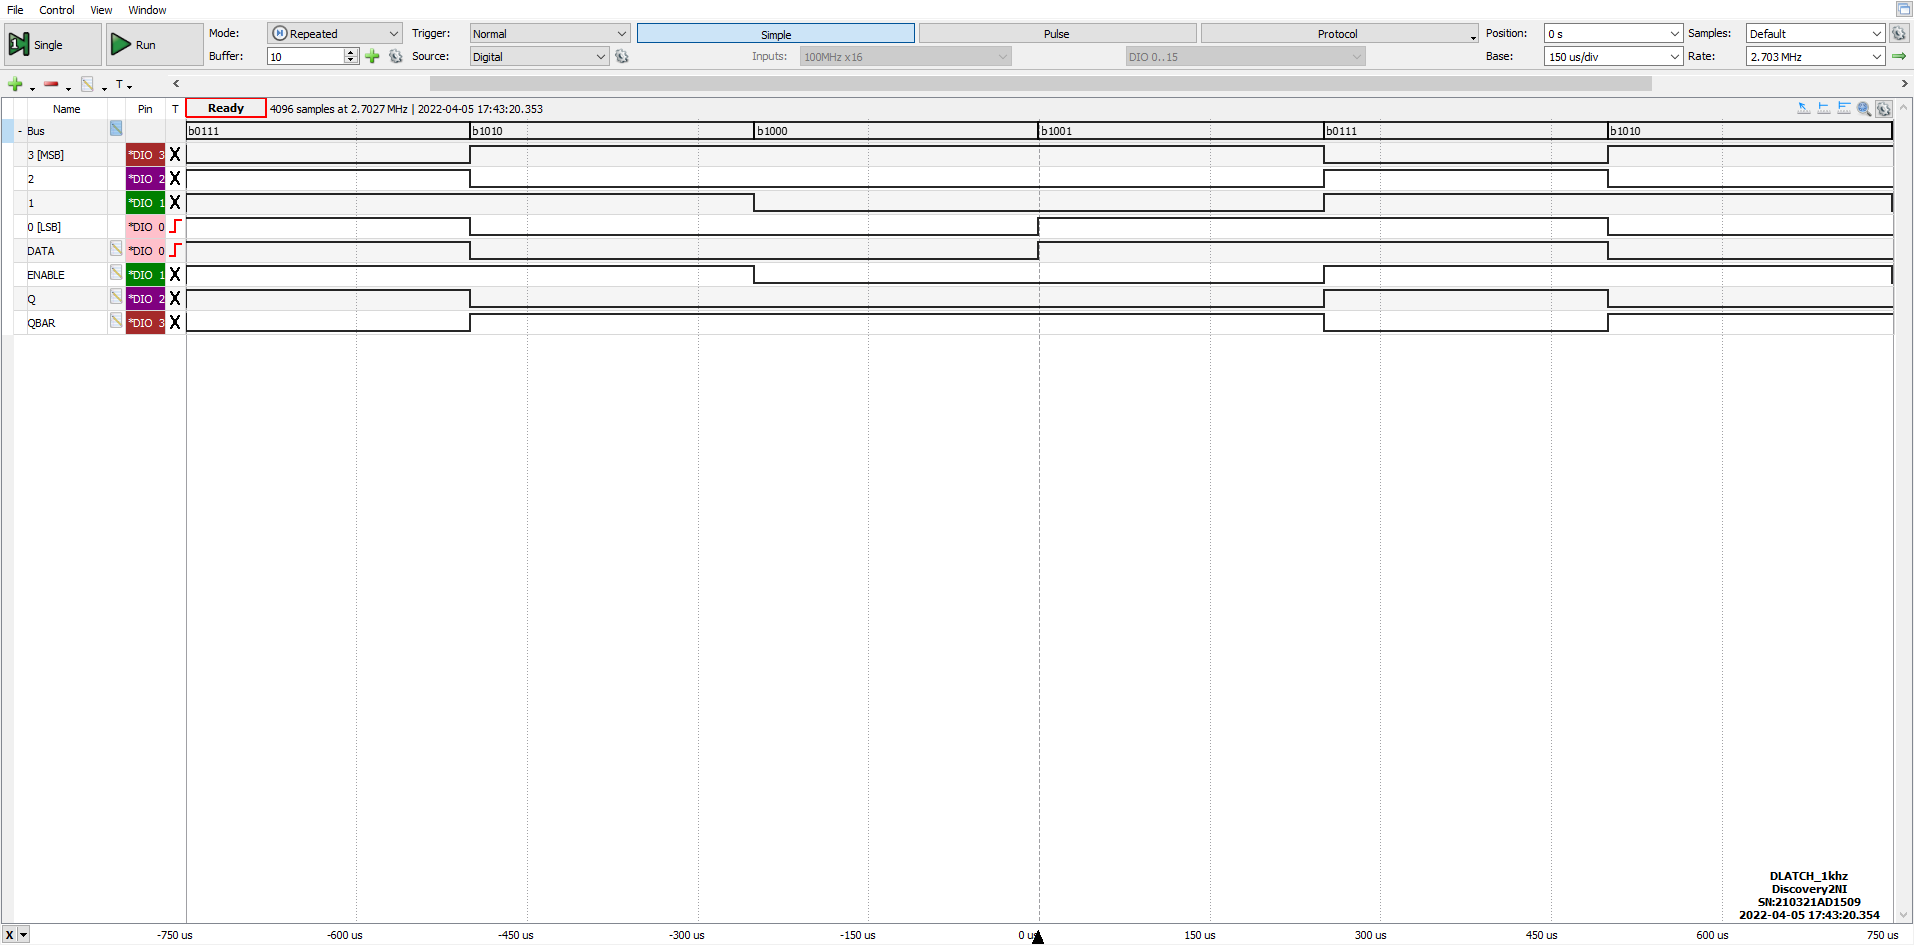
\includegraphics[width=\textwidth]{dlatch}
    \caption{Acquisizione di un ciclo completo (frequenza 1 kHz) con Logic
    Analyzer dei segnali in ingresso ($D =$ DIO 0, $E =$ DIO 1) e in uscita
    ($Q =$ DIO 2, $\overline{Q} =$ DIO 3) dal D-Latch.
    \label{fig: dlatch}}
\end{figure}

Dalla \cref{fig: dlatch} si osserva come durante lo stato basso di Enable
il segnale in uscita rimanga costante rispetto a variazioni del segnale in
$D$, mentre quando $E = 1 \implies Q(t + \Delta t) = D$ coerentemente con
quanto previsto dalla tabella di verità.

\subsection{Misura dei tempi del ritardo nelle transizioni di stato}
Si riescono a distinguere due diverse transizioni dei segnali in ingresso per
ciascun valore di sfasamento tra i due segnali di clock in $D$ ed $E$;
per $\phi = \SI{90}{\degree}$:
\begin{enumerate}
\item $D: 1 \to 0$, $E \coloneqq 1$ \label{item: Dfall}
\item $D \coloneqq 1$, $E: 0 \to 1$. \label{item: Erise}

Mentre per $\phi = - \SI{90}{\degree} = 270 \; \si{\degree}$:
\item $D \coloneqq 0$, $E: 0 \to 1$ \label{item: Efall}
\item $D: 0 \to 1$, $E \coloneqq 1$. \label{item: Drise}
\end{enumerate}


Il ritardo di durata maggiore appare quello della transizione dell'input D da alto a basso ($40$ ns $\pm 10$ ns).

Dalle misure prese con i cursori dell'oscilloscopio (a cui associamo come
incertezza il contributo dato dalle specifiche del datasheet, tenendo conto
dell'instabilità delle tracce sullo schermo) troviamo
\begin{align*}
    t_{PLH}= 5.2 \pm 1.2 \; \si{n\s} \\
    t_{PHL}= 25 \pm 2 \; \si{n\s}
\end{align*}

Dalle specifiche del DS si trova che i tempi di propagazione tipici e massimi
per una singola porta NAND sono:
\begin{table}[htbp]
\centering
\begin{tabular}{cccc}
	& typ & max & [units] \\
    $t\ped{PLH}$ & $11$ & $22$ & \si{n\s} \\
    $t\ped{PHL}$ & $7$ & $15$ & \si{n\s}
\end{tabular}
\end{table}

%=======================
\section{Shift-register con edge-triggered D-Flip Flop}
\subsection{Costruzione del circuito}
\subsection{Verifica della sincronia delle uscite}
\subsection{Studio delle commutazioni di stato in uscita}
\subsection{Studio del canale di ingresso con Preset e D-switch attivi}
\subsection{Contatore BCD con Flip Flop in cascata}

Dalle specifiche del DS risulta quindi che 
\begin{align*}
    I\ped{IH, max}= -0.4 \; \si{m\A} \\
    I\ped{OH, max}= 40 \; \si{\micro\A} \\
    \text{FO} = 10
\end{align*}
A questo punto abbiamo preparato l'amperometro utilizzando il fondoscala da 2 mA viste le entità delle correnti che andremo a misurare: per prima cosa misureremo la corrente $I_{IH,max}$ per entrambi i due integrati, montando l'amperometro in serie tra l'ingresso della porta logica e l'uscita di WaveGen 1 dell'AD2. Quindi abbiamo inviato all'uscita WG1 una tensione DC pari a 5V.
\begin{gather*}
    I_{IH,1}=16 \pm 1 \mu A\\
    I_{IH,2}=10 \pm 1 \mu A\\   
\end{gather*}
Che risultano essere compatibili entro i limiti del datasheet.
Arrivati a questo punto abbiamo rimosso l'amperometro e abbiamo inviato all'ingresso della porta un segale DC a 0 V sempre utilizzando l'uscita WG1, e abbiamo inserito un potenziometro da $10 \; k\ohm$ in serie all'uscita della stessa porta logica utilizzata in precedenza, misurando la corrente che scorre attraverso questo quando la tensione in uscita dalla porta è pari a $3.40 \pm 0.03 \; V$.
\begin{gather*}
    I_{OH,1}=495 \pm 4 \mu A\\
    I_{OH,2}=315 \pm 3 \mu A\\   
\end{gather*}
%TODO inseirire cosa sarebbe successo se avessi abbassato la tensione in uscita fino a 2.5 V circa
Da questo si ricava che:
\begin{gather*}
    \mbox{Fan-out}_1=31 \pm 2\\
    \mbox{Fan-out}_2=32 \pm 3\\
\end{gather*}
Valori che sono notevolmente più alti delle aspettative e non compatibili con esse, ma risultano essere compatibili tra di loro.

\section{Generatore di sequenze pseudo-casuali}
\subsection{Costruzione del circuito}
\subsection{Analisi e verifica del funzionamento}
\subsection{Studio delle sequenze generabili con diverse condizioni iniziali}

%=======================
\section{Divisori di frequenza con contatori binari}
\subsection{Costruzione del circuito}
\subsection{Verifica del ciclo di funzionamento dei contatori}
\subsection{Verifica della divisione in frequenza}
\subsection{Transizione sincrona del contatore}
\subsection{Costruzione di un divisore di frequenza 1/10}
\subsection{Divisore di frequenza programmabile con RCO}
\subsection{Misura dei tempi caratteristici del divisore RCO}
\subsection{Analisi e verifica del comportamento del divisore RCO}

%=======================
\section{Sintetizzatore musicale}

%=======================
\section*{Conclusioni e commenti finali}
Si è riusciti a verificare il corretto comportamento delle porte TTL studiate
caratterizzandone le tensioni, correnti di operazione e tempi caratteristici
di circuiti integrati come il SN7404.
Inoltre, è stato possibile verificare il funzionamento di circuiti logici di
diversa complessità costruiti con porte NAND, XOR, e OR e si è riusciti ad
apprezzare l'effetto dei tempi di propagazione delle porte nella conversione
dalla codifica Gray al binario.

%=======================
\section*{Dichiarazione}
I firmatari di questa relazione dichiarano che il contenuto della relazione \`e
originale, con misure effettuate dai membri del gruppo, e che tutti i firmatari
hanno contribuito alla elaborazione della relazione stessa.

\end{document}
